\documentclass[12pt]{article}
\usepackage[left=1cm, right=1cm, top=2cm,bottom=1.5cm]{geometry} 

\usepackage[parfill]{parskip}
\usepackage[utf8]{inputenc}
\usepackage[T2A]{fontenc}
\usepackage[russian]{babel}
\usepackage{enumitem}
\usepackage[normalem]{ulem}
\usepackage{amsfonts, amsmath, amsthm, amssymb, mathtools}
\usepackage{tabularx}
\usepackage{hhline}

\usepackage{accents}
\usepackage{fancyhdr}
\pagestyle{fancy}
\renewcommand{\headrulewidth}{1.5pt}
\renewcommand{\footrulewidth}{1pt}

\usepackage{graphicx}
\usepackage[figurename=Рис.]{caption}
\usepackage{subcaption}
\usepackage{float}

%%Наименование папки откуда забирать изображения
\graphicspath{ {./images/} }

%%Изменение формата для ввода доказательства
\renewcommand{\proofname}{$\square$  \nopunct}
\renewcommand\qedsymbol{$\blacksquare$}

%%Изменение отступа на таблицах
\addto\captionsrussian{%
	\renewcommand{\proofname}{$\square$ \nopunct}%
}
%% Римские цифры
\newcommand{\RN}[1]{%
	\textup{\uppercase\expandafter{\romannumeral#1}}%
}

%% Для удобства записи
\newcommand{\MR}{\mathbb{R}}
\newcommand{\MQ}{\mathbb{Q}}
\newcommand{\MN}{\mathbb{N}}
\newcommand{\MI}{\mathrm{I}}
\newcommand{\MJ}{\mathrm{J}}
\newcommand{\MH}{\mathrm{H}}
\newcommand{\MT}{\mathrm{T}}
\newcommand{\MU}{\mathcal{U}}
\newcommand{\MV}{\mathcal{V}}
\newcommand{\MW}{\mathcal{W}}
\newcommand{\VN}{\varnothing}
\newcommand{\VE}{\varepsilon}

\theoremstyle{definition}
\newtheorem{defn}{Опр:}
\newtheorem{rem}{Rm:}
\newtheorem{prop}{Утв.}
\newtheorem{exrc}{Упр.}
\newtheorem{lemma}{Лемма}
\newtheorem{theorem}{Теорема}
\newtheorem{corollary}{Следствие}

\newenvironment{cusdefn}[1]
{\renewcommand\thedefn{#1}\defn}
{\enddefn}

\DeclareRobustCommand{\divby}{%
	\mathrel{\text{\vbox{\baselineskip.65ex\lineskiplimit0pt\hbox{.}\hbox{.}\hbox{.}}}}%
}
%Короткий минус
\DeclareMathSymbol{\SMN}{\mathbin}{AMSa}{"39}
%Длинная шапка
\newcommand{\overbar}[1]{\mkern 1.5mu\overline{\mkern-1.5mu#1\mkern-1.5mu}\mkern 1.5mu}
%Функция знака
\DeclareMathOperator{\sgn}{sgn}

%Функция ранга
\DeclareMathOperator{\rk}{\text{rk}}

%Обозначение константы
\DeclareMathOperator{\const}{\text{const}}

%Интеграл в большом формате
\DeclareMathOperator{\dint}{\displaystyle\int}

\newcommand{\smallerrel}[1]{\mathrel{\mathpalette\smallerrelaux{#1}}}
\newcommand{\smallerrelaux}[2]{\raisebox{.1ex}{\scalebox{.75}{$#1#2$}}}

\newcommand{\smallin}{\smallerrel{\in}}
\newcommand{\smallnotin}{\smallerrel{\notin}}

\newcommand*{\medcap}{\mathbin{\scalebox{1.25}{\ensuremath{\cap}}}}%
\newcommand*{\medcup}{\mathbin{\scalebox{1.25}{\ensuremath{\cup}}}}%

\makeatletter
\newcommand{\vast}{\bBigg@{3.5}}
\newcommand{\Vast}{\bBigg@{5}}
\makeatother

%Скалярное произведение
\DeclarePairedDelimiterX{\inner}[2]{\langle}{\rangle}{#1, #2}

%Подпись символов снизу
\newcommand{\ubar}[1]{\underaccent{\bar}{#1}}

\begin{document}
\lhead{Математический анализ - \RN{2}}
\chead{Шапошников С.В.}
\rhead{Лекция - 19}
\section*{Условный экстремум}
В прошлый раз мы рассматривали задачу на условный экстремум:
$$
	\left\{
	\begin{array}{l}
		f(x) \to \text{extr}!\\
		x \in l
	\end{array}
	\right.
$$
где предполагали $f \colon \MR^n \to \MR$. Для её решения мы начали рисовать множества уровня: $f(x) = f_0$ и искали решение там, где линия уровня $f$ касалась бы линии, которая задает нам условие.

\textbf{\uline{Идея}}: Ищем экстремумы в тех точках, в которых линии уровня исследуемой функции касаются линии задающей условия.

\textbf{\uline{Задача}}: Типичной задачей рассматривали поиск экстремума на единичной окружности:
$$
	\left\{
	\begin{array}{l}
		x + y \to \text{extr}!\\
		x^2 + y^2  = 1
	\end{array}
	\right.
$$
В этом случае рисуем окружность, проводим линии уровня и смотрим точки соприкосновения.
\begin{figure}[H]
	\centering
	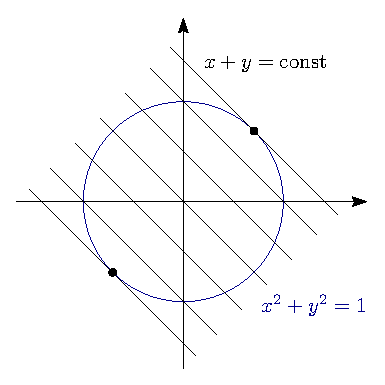
\includegraphics[width=0.35\textwidth]{19_1.eps}
	\caption{Поиск точек экстремума на окружности.}
	\label{19_1}
\end{figure}
Для того, чтобы разобраться с теорией условных экстремумов, оставляя при этом доступную геометрическую интерпритацию, для начала исследуем некоторые геометрические объекты.

\newpage
\section*{Гладкие поверхности}
\begin{defn}
	Множество $M^k \subset \MR^n$ называется \uwave{гладкой $k$-мерной поверхностью}, если $\forall p \in M^k$ найдутся окрестности $Q(p)_x \subset \MR^n, \, V(0)_u \subset \MR^n$ и диффеоморфизм $f \colon Q \to V$ такой, что:
	$$
		f\big(M^k \cap Q(p)_x\big) = V(0)_u \cap \{u_{k+1} = \dotsc = u_n = 0\}
	$$
\end{defn}

Попробуем визуализировать это понятие.
\begin{figure}[H]
	\centering
	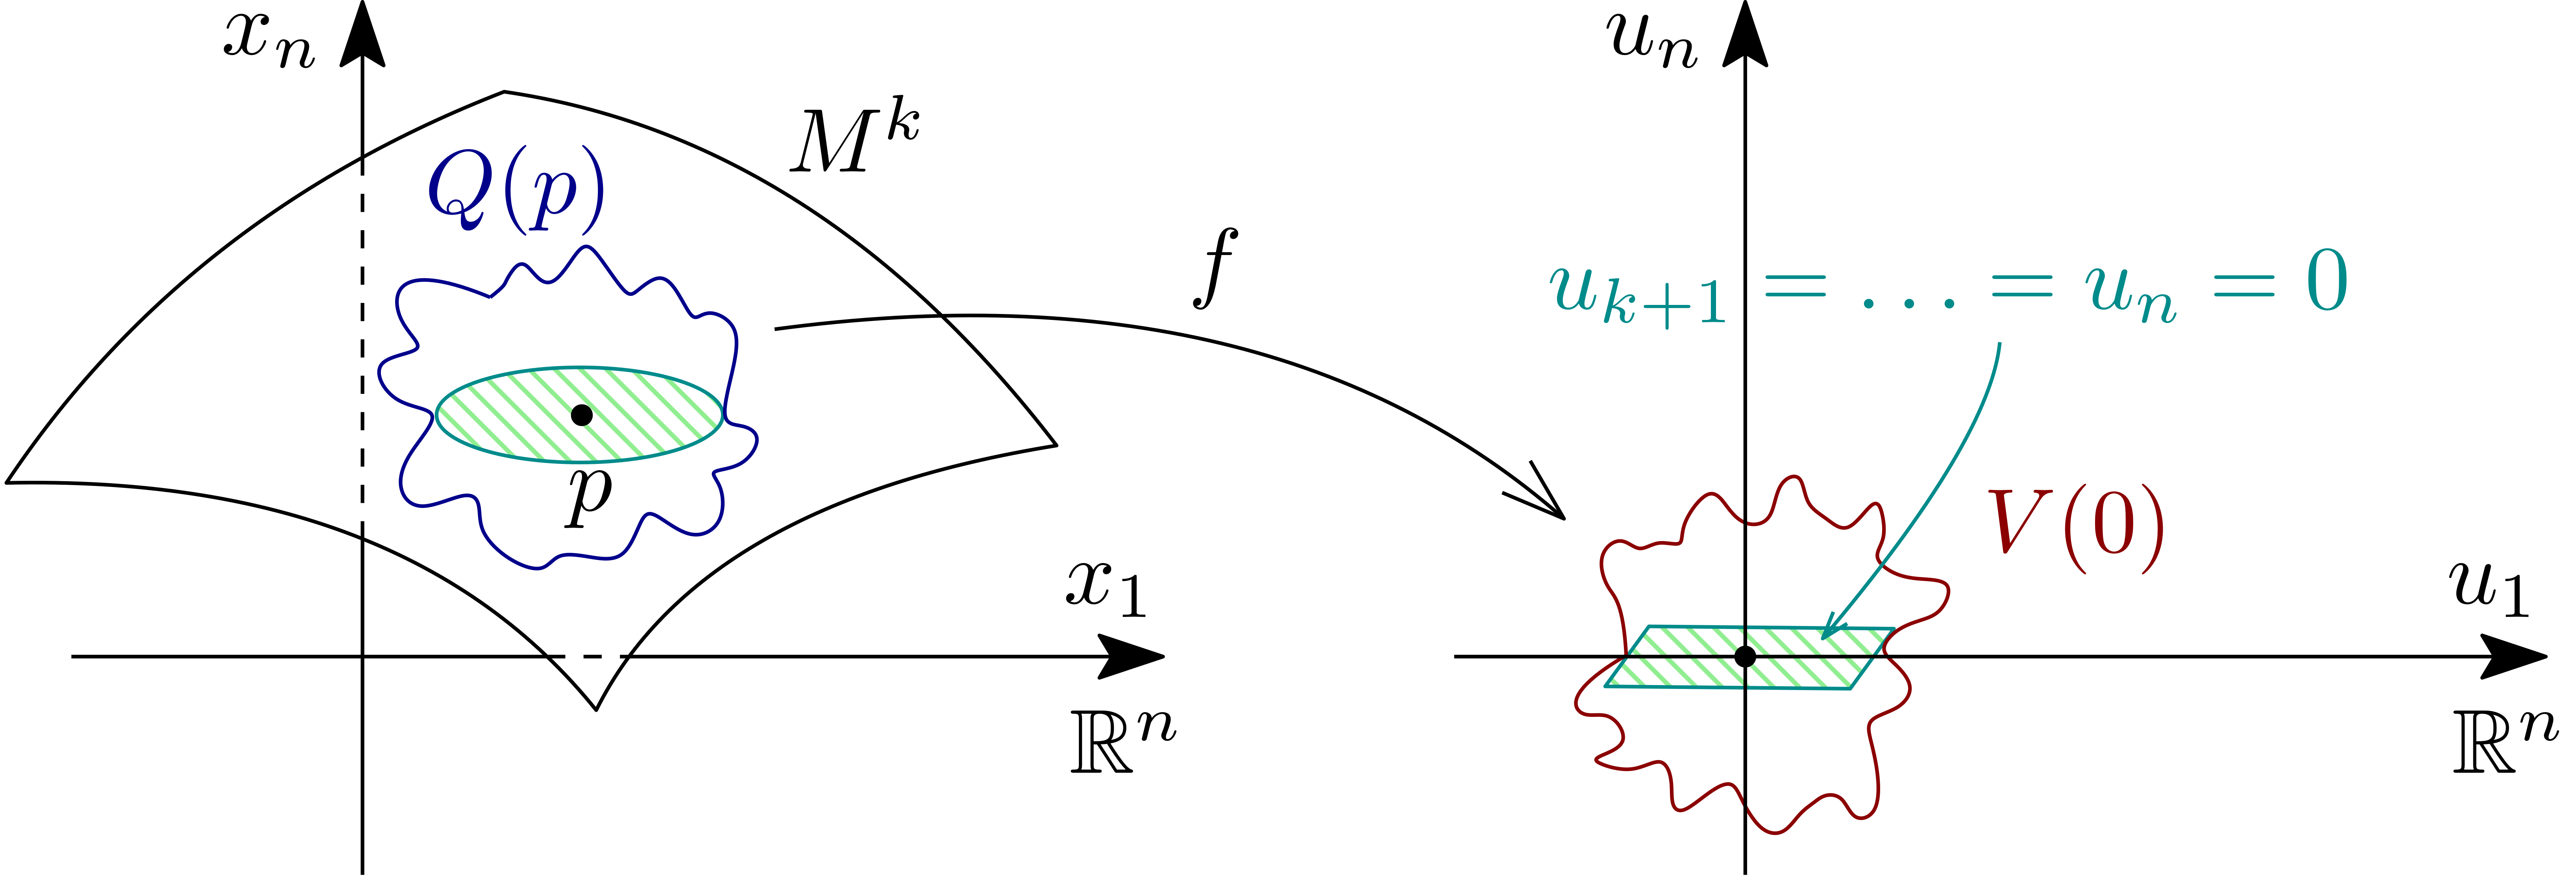
\includegraphics[width=0.75\textwidth]{19_2.png}
	\caption{Определение гладкой $k$-мерной поверхности.}
	\label{19_2}
\end{figure}
То есть, гладкая $k$-мерная поверхность это такая поверхность, которую локально можно спрямить в $k$-мерную плоскость с помощью диффеоморфизма. 
\begin{rem}
	В определении ничего не говорится про дополнительные свойства множества, только про то, что это подмножество $\MR^n$, которое локально выпрямляется в $k$-мерную плоскость.
\end{rem}
Заметим что этот объект мы уже встречали в виде множества решений уравнений, которое исследовалось в теореме о неявной функции $\Rightarrow$ оно является $k$-мерной поверхностью. Например, знаем что $\tfrac{\partial F}{\partial y} \neq 0$ и пусть $\{F(x,y) = 0\} \neq \VN$, тогда:
$$
	\{F(x,y) = 0\} = M^1 \subset \MR^2
$$
\begin{figure}[H]
	\centering
	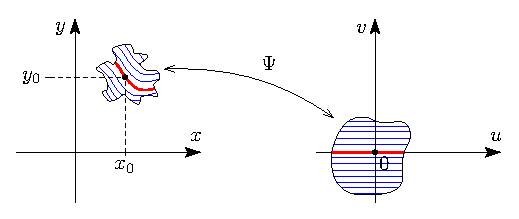
\includegraphics[width=0.65\textwidth]{19_3.eps}
	\caption{Выпрямление кривой линии в одномерную прямую.}
	\label{19_3}
\end{figure}
Следовательно, кривая в $\MR^2$ которую можно выпрямить - это гладкая одномерная поверхность.
\begin{prop}
	$M^k$ - гладкая $k$-мерная поверхность $\Leftrightarrow \forall p \in M^k, \, \exists \, \MW(p)$, непрерывно дифференцируемые в ней функции $F_{k+1}, \dotsc, F_n$ такие, что $dF_{k+1}, \dotsc, dF_n$ - линейно независимы и выполнено следующее:
	$$
		M^k \cap \MW(p) = \{x \in \MW(p) \mid F_{k+1}(x) = 0, \dotsc, F_n(x) = 0\}
	$$
\end{prop}
\begin{rem}
	Линейно независимые дифференциалы это то же самое, что и линейно независимые градиенты (т.е. задающие дифференциалы векторы). В случае одного $n$ требуется невырожденность градиента.
\end{rem}
Таким образом, любая $k$-мерная плоскость может быть задана, как множество решений $(n-k)$ линейных уравнений: Всякая двумерная плоскость в пространстве задается как множество решений из одного уравнения, всякая прямая в пространстве задается как решение системы из двух уравнений и так далее.

\textbf{Пример}: $\MR^3, \, F(x,y,z) = 0$, функция невырождена (градиент у неё нигде не ноль). Если множество не пустое, то мы получили гладкую $k$-мерную поверхность. Сфера, конус, парабалоиды, гиперболоиды будут двумерными гладкими поверхностями (кроме особых точек). И наоборот, мы можем смотреть на решение системы уравнений, как на гладкую $k$-мерную поверхность.

\begin{proof}\hfill\\
	$(\Leftarrow)$ Условие независимости $dF_{k+1}, \dotsc, dF_n$ по-другому можно сформулировать так: 
	$$\rk{
		\begin{pmatrix}
			\tfrac{\partial F_{k+1}}{\partial x_1} & \dotsc & \tfrac{\partial F_{k+1}}{\partial x_n} \\
			\vdots & \ddots & \vdots \\
			\tfrac{\partial F_n}{\partial x_1} & \dotsc & \tfrac{\partial F_n}{\partial x_n}
		\end{pmatrix}} = n-k 
	$$ 
	то есть, $(n-k)$ строчек этой матрицы линейно независимы. Тогда с точностью до нумерации координат можно написать, что минор порядка $(n-k)$ не равен нулю:
	$$
		\begin{vmatrix}
			\tfrac{\partial F_{k+1}}{\partial x_{k+1}} & \dotsc & \tfrac{\partial F_{k+1}}{\partial x_n} \\
			\vdots & \ddots & \vdots \\
			\tfrac{\partial F_n}{\partial x_{k+1}} & \dotsc & \tfrac{\partial F_n}{\partial x_n}
		\end{vmatrix} \neq 0
	$$
	По условию, $p \in M^k\cap \MU(p) \Rightarrow F_{k+1}(p) = \dotsc = F_n(p) = 0$.
	Тогда для следующей системы уравнений:
	$$
		\left\{
			\begin{array}{ccc}
				F_{k+1}(x_1,\dotsc , x_k, x_{k+1}, \dotsc, x_n) & = & 0\\
				\vdots & \vdots & \vdots \\
				F_n(\underbrace{x_1,\dotsc, x_k}_{\widetilde{x}}, \underbrace{x_{k+1}, \dotsc, x_n}_{\widetilde{y}}) & = & 0
			\end{array}
		\right.
	$$
	выполняются условия теоремы о неявной функции $\Rightarrow$ можем указать замену координат, которая множество решений этой системы в окрестности точки $p$ превращает в пересечение открытой окрестности и плоскости, где координаты $\overline{k+1, n}$ равны нулю: 
	$$
		f \colon \left\{
		\begin{array}{lcl}
			w_i& = &\widetilde{x}_i - p_i, \, i = \overline{1,k} \\
			w_j& = &F_j(\widetilde{x},\widetilde{y}), \, j = \overline{k+1,n}
		\end{array}\right., \, f(p) = 0
	$$
	Далее, аналогично доказательству теоремы о неявной функции, найдутся окрестности $Q(p) \subset \MW(p)$ и $V(0)$ такие, что $f \colon Q(p) \to V(0)$ - локальный диффеоморфизм. Причем, по условию: 
	$$
		M^k \cap Q(P) \subset M^k \cap \MW(p) \Rightarrow 	M^k \cap Q(p) = \{x \in Q(p) \mid F_{k+1}(x) = 0, \dotsc, F_n(x) = 0\}
	$$
	Тогда аналогично теореме о неявной функции можно проверить, что:
	$$
		f\big(M^k \cap Q(p)\big) = V(0) \cap \{w_{k+1} = \dotsc = w_n = 0\} = \{w \in V(0) \mid w_{k+1} = \dotsc = w_n = 0 \}
	$$
	\begin{proof}\hfill\\
		$(\Rightarrow)$ Под действием отображения $f$ верно: $
			\left\{
			\begin{array}{lcl}
				w_i& = &\widetilde{x}_i - p_i, \, i = \overline{1,k} \\
				w_j& = &F_j(\widetilde{x},\widetilde{y}), \, j = \overline{k+1,n}
			\end{array}\right.
		$, тогда получим следующее: 
		$$
			(\widetilde{x},\widetilde{y}) \in M^k \cap Q(p) \Rightarrow w \in V(0), \, \left\{
			\begin{array}{lcl}
				w_i& = &\widetilde{x}_i - p_i, \, i = \overline{1,k} \\
				w_j& = &F_j(\widetilde{x},\widetilde{y}) = 0, \, j = \overline{k+1,n}
			\end{array}\right.
		$$
		
		$(\Leftarrow)$ По определению диффеоморфизма, каждая точка из $V(0)$ есть образ какой-то точки из $Q(p)$. Получается, что: 
		$$
			\forall w \in V(0), \, \exists \, (\widetilde{x},\widetilde{y}) \in Q(p) \colon \left\{
				\begin{array}{lcl}
					w_i& = &\widetilde{x}_i - p_i, \, i = \overline{1,k} \\
					w_j& = &F_j(\widetilde{x},\widetilde{y}), \, j = \overline{k+1,n}
				\end{array}
			\right.
		$$
		Но поскольку $w_{k+1} = \dotsc = w_n = 0$ и $w \in V(0) \Rightarrow (\widetilde{x},\widetilde{y}) \in Q(p), \, F_{k+1}(\widetilde{x},\widetilde{y}) = \dotsc = F_n(\widetilde{x},\widetilde{y}) = 0$.
	\end{proof}
	Простоты ради, можно было определить замену:
	$$
		f \colon \left\{
		\begin{array}{ccc}
			u^\prime_1 + p_1 = u_1 & = &\widetilde{x}_1 \\
			\vdots & \ddots & \vdots \\
			u^\prime_k + p_k = u_k & = &\widetilde{x}_k \\
			v_1& = &F_{k+1}(\widetilde{x},\widetilde{y}) \\
			\vdots & \ddots & \vdots \\
			v_{n-k}& = &F_n(\widetilde{x},\widetilde{y})
		\end{array}\right. \Leftrightarrow  
		\left\{
		\begin{array}{lcl}
			u& = &\widetilde{x} \\
			v& = &F(\widetilde{x},\widetilde{y})
		\end{array}\right.
	$$
	И в этом случае использовать доказательство теоремы о неявной функции, где $Q(p) = \MU^\prime(0) \times \MV(\widetilde{y}_0)$, $V(0) = f\big(Q(p)\big)$ и $p = (\widetilde{x}_0, \widetilde{y}_0)$. Тогда автоматически получим:
	$$
		f\big(\{(\widetilde{x},\widetilde{y}) \mid \widetilde{x} \in \MU(\widetilde{x}_0), \, \widetilde{y} \in \MV(\widetilde{y}_0), \, F(\widetilde{x},\widetilde{y}) = 0 \}\big) = \{(u,v) \mid u \in \MU(\widetilde{x}_0), \, v = 0 \} \Leftrightarrow
	$$
	$$
		 \Leftrightarrow f\big(\{(\widetilde{x},\widetilde{y}) \mid \widetilde{x} \in \MU^\prime(0), \, \widetilde{y} \in \MV(\widetilde{y}_0), \, F(\widetilde{x},\widetilde{y}) = 0 \}\big) = \{(u^\prime,v) \mid u^\prime \in \MU(0), \, v = 0 \} \Leftrightarrow
	$$
	$$
		\Leftrightarrow f\big(\{(\widetilde{x},\widetilde{y}) \mid (\widetilde{x},\widetilde{y}) \in Q(p), \, F(\widetilde{x},\widetilde{y}) = 0 \}\big) = \{(u^\prime,v) \mid (u^\prime,v) \in V(0), \, v = 0 \} 
	$$
	
	$(\Rightarrow)$ По определению гладкой $k$-мерной поверхности, $\forall p \in M^k$ найдутся окрестности $Q(p), V(0)$ и диффеоморфизм $f \colon Q \to V$ такой, что:
	$$
		f\big(M^k \cap Q(p)\big) = V(0) \cap \{u_{k+1} = \dotsc = u_n = 0\}
	$$
	\begin{figure}[H]
		\centering
		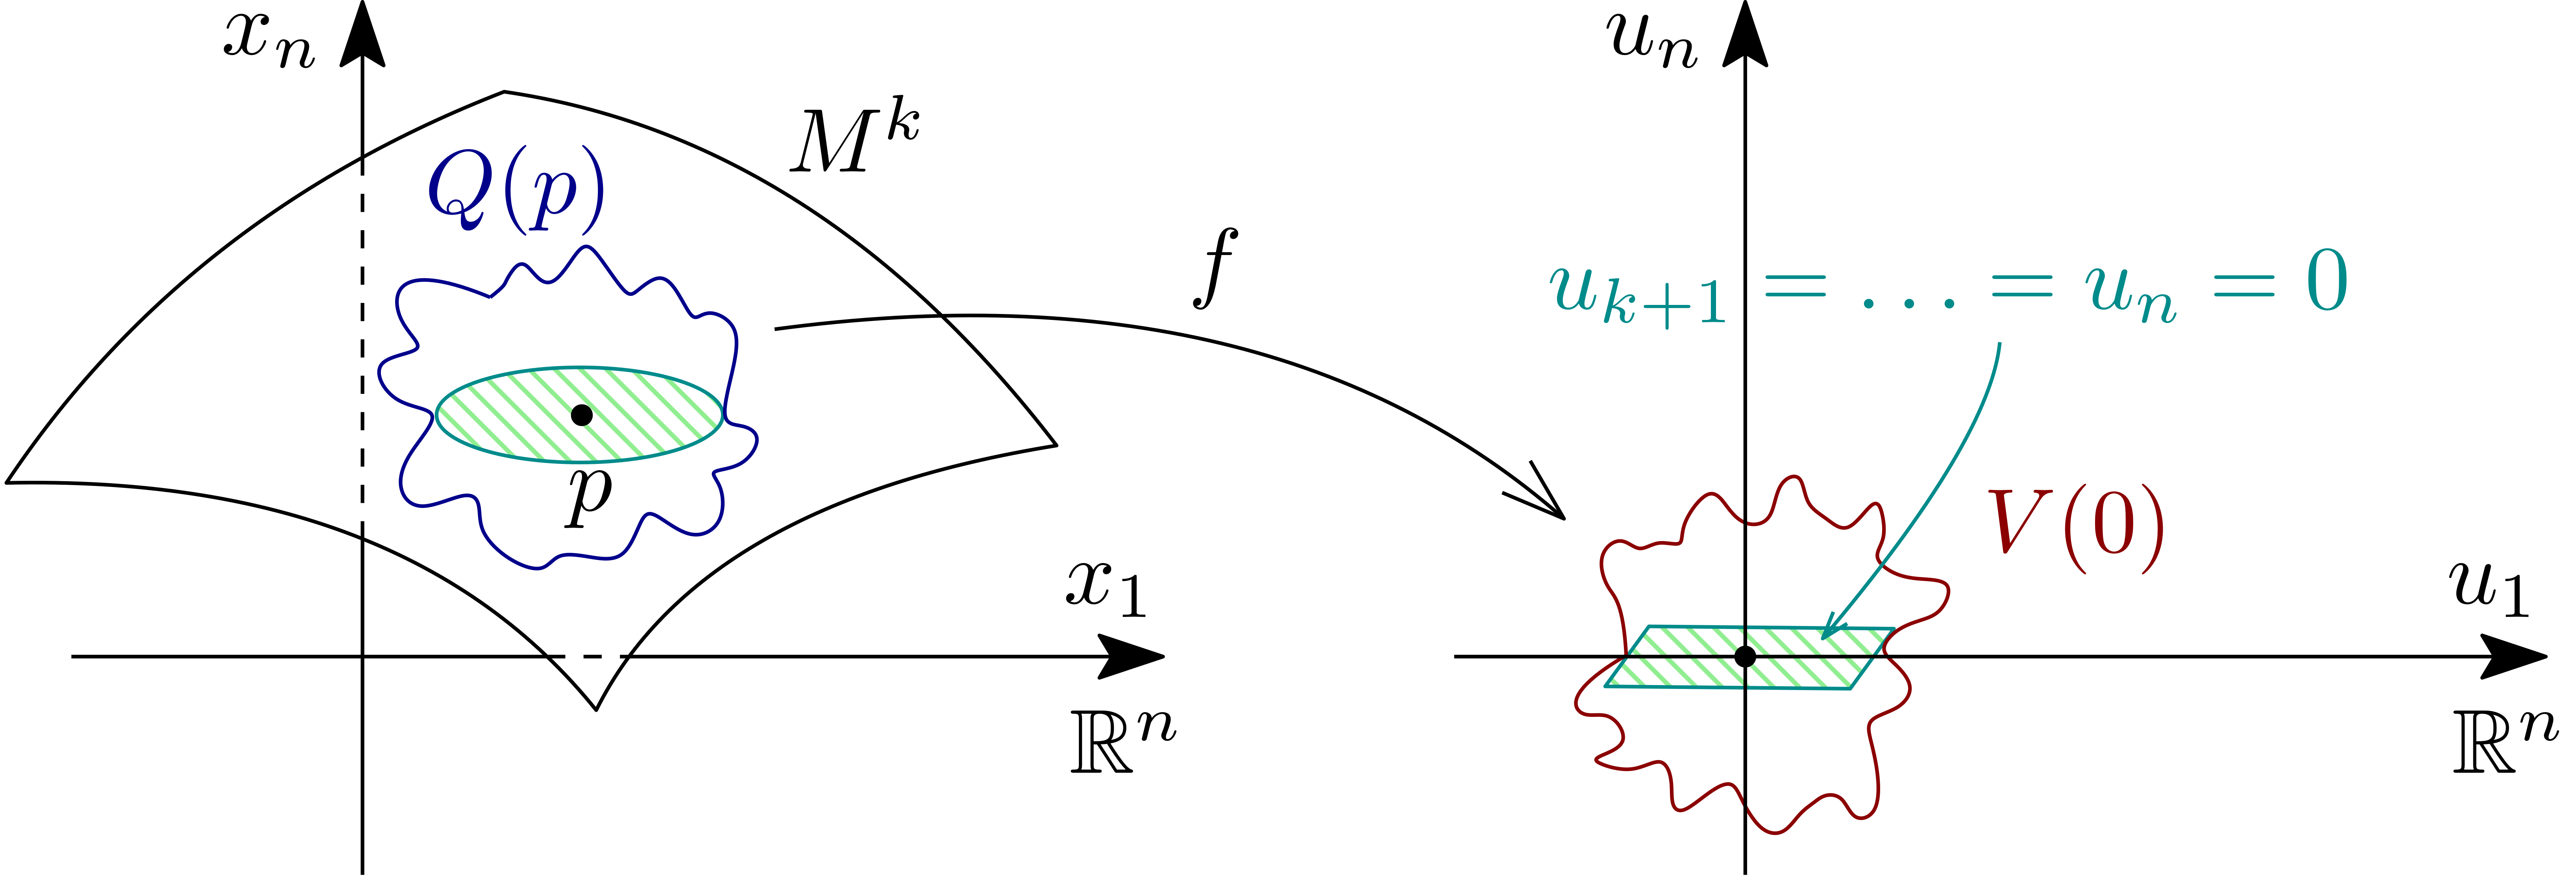
\includegraphics[width=0.75\textwidth]{19_2.png}
		\caption{Определение гладкой $k$-мерной поверхности.}
		\label{19_4}
	\end{figure}
	Хотим найти функции $F_{k+1}, \dotsc, F_n$, чтобы они задавали кусок $M^k \cap Q(p)$ как решение следующей системы уравнений: $F_{k+1}(x) = \dotsc = F_n(x) = 0$. Возьмем $F_m(x) = u_m$ - функции, которые задают диффеоморфизм:
	$$
		f \colon \left\{
		\begin{array}{ccc}
			u_1& = &F_1(x) \\
			\vdots & \vdots & \vdots \\
			u_n& = &F_n(x)
		\end{array}\right.
	$$
	Множество $M^k \cap Q(p)$ представляет собой ровно те точки, которые под действием диффеоморфизма $f$ перешли в точки $V(0) \cap \{u_{k+1} = \dotsc = u_n = 0\}$, то есть в которых: 	
	$$
		\left\{
		\begin{array}{ccccc}
			F_{k+1}(x) & = & u_{k+1} &=& 0\\
			\vdots & \vdots & \vdots & \vdots & \vdots \\
			F_n(x)& = &u_n &=& 0
		\end{array}\right.
	$$
	Таким образом, мы получили $u_m = f(F_m) = F_m$ и по инвариантности $\RN{1}$-го дифференциала мы получим:
	$$
		du_m = \dfrac{\partial u_m}{\partial F_{k+1}}dF_{k+1} + \dotsc + \dfrac{\partial u_m}{\partial F_m}dF_m + \dotsc + \dfrac{\partial u_n}{\partial F_n}dF_n = 1{\cdot}dF_m = dF_m
	$$
	Следовательно, если бы оказались линейно зависимыми $dF_{k+1}, \dotsc, dF_n$, тогда оказались бы линейно зависимыми и $du_{k+1}, \dotsc, du_n$ в системе координат $u_1, \dotsc, u_n$, что невозможно в силу того, что градиенты этих функций имеют вид:
	$$
		\begin{pmatrix}
			\nabla u_{k+1} \\
			\vdots \\
			\nabla u_n
		\end{pmatrix} = 
		\begin{pmatrix}
			0 & \dotsc & 0 & 1 & \dotsc & 0 \\
			\vdots & \ddots & \vdots & \vdots & \ddots & \vdots \\
			0 & \dotsc & 0 & 0 & \dotsc & 1
		\end{pmatrix}
	$$
	То есть они линейно независимы.
\end{proof}

\begin{prop}
	$M^k$ - гладкая $k$-мерная поверхность $\Leftrightarrow$ в окрестности всякой своей точки $M^k$ является графиком дифференцируемой функции $\MR^k \to \MR^{n-k}$.
\end{prop}
\textbf{Пример}: $M^2 \subset \MR^3$, в окрестности всякой своей точки это множество является графиком функции либо $z = f(x,y)$, либо $y = f(x,z)$, либо $x = f(y,z)$.
\begin{figure}[H]
	\centering
	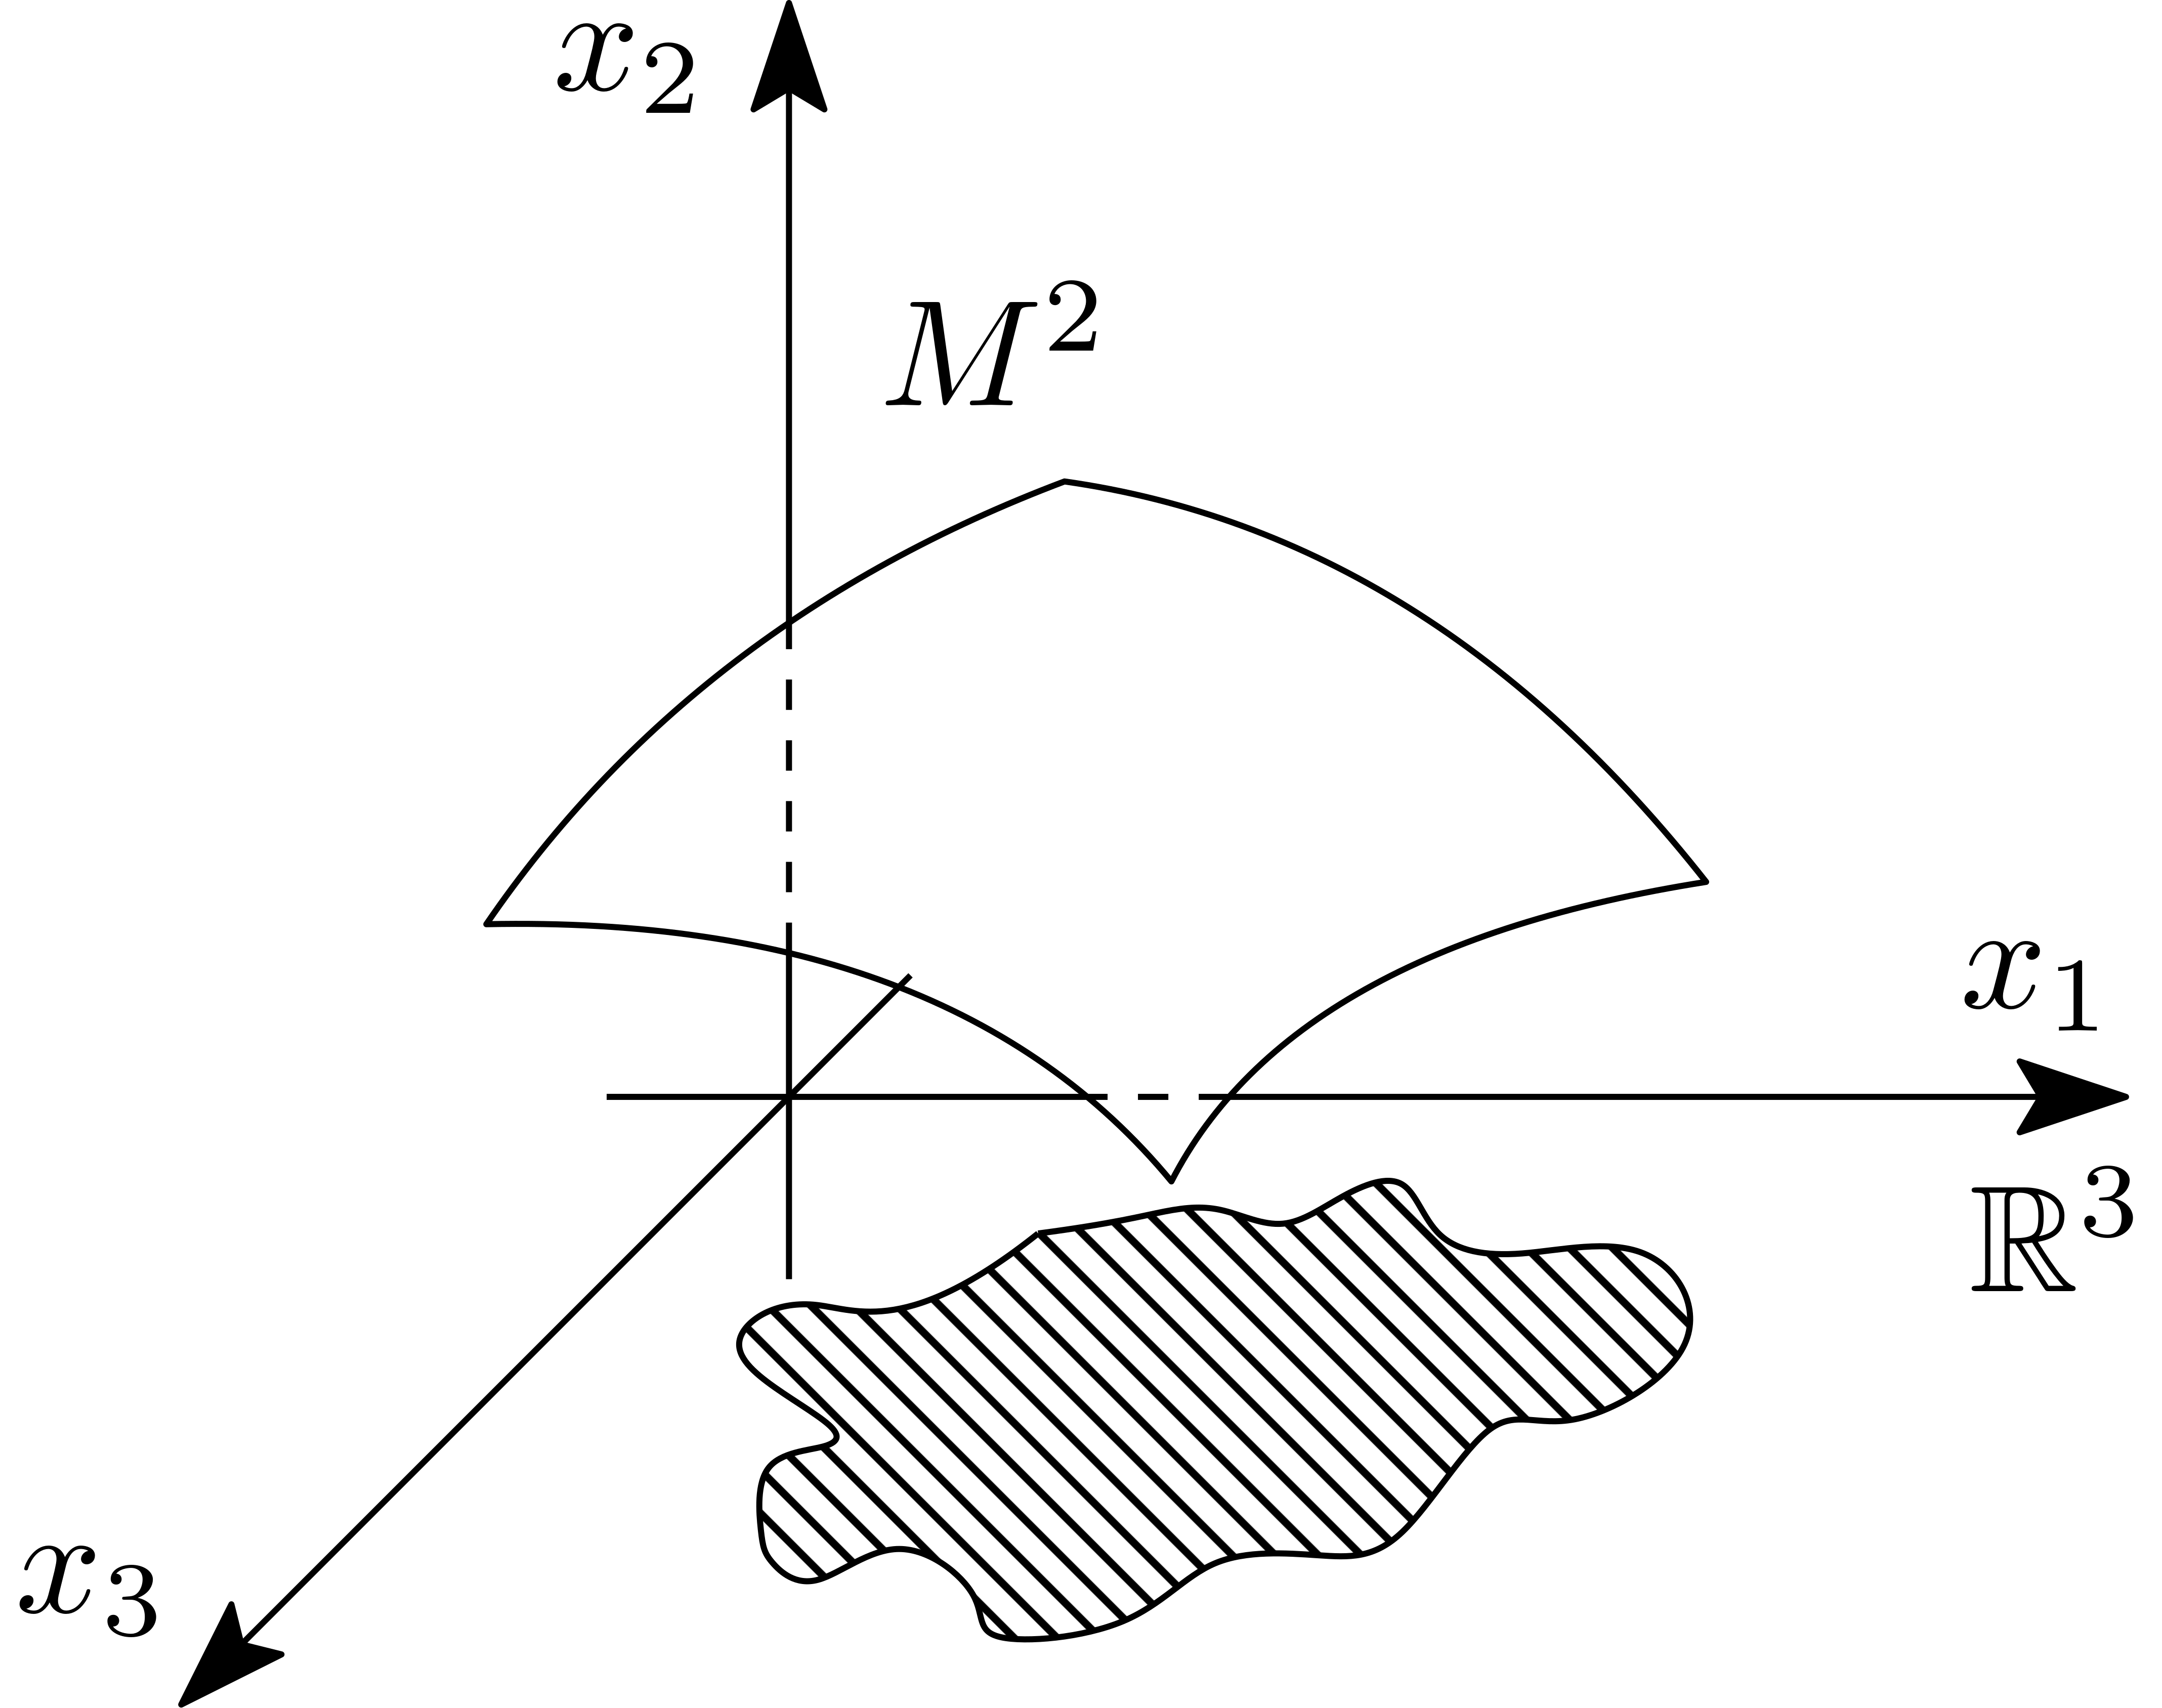
\includegraphics[width=0.35\textwidth]{19_5.png}
	\caption{Гладкая $2$-мерная поверхность в пространстве.}
	\label{19_5}
\end{figure}
\begin{rem}
	Таким образом, гладкая $k$-мерная поверхность это что-то составленное из лоскутков в виде графиков отображений. Это опять напоминает теорему о неявной функции.
\end{rem}

\textbf{Пример}: $M^1 \subset \MR^3$, в окрестности всякой своей точки это множество является графиком функции, который задается как:
$$
	\left\{ 
		\begin{array}{ccc}
			z & = & f_1(x)\\
			y & = & f_2(x)
		\end{array}
	\right.
	\vee
	\left\{ 
		\begin{array}{ccc}
			x & = & f_1(z)\\
			y & = & f_2(z)
		\end{array}
	\right.
	\vee
	\left\{ 
		\begin{array}{ccc}
			x & = & f_1(y)\\
			z & = & f_2(y)
		\end{array}
	\right.
$$
\begin{figure}[H]
	\centering
	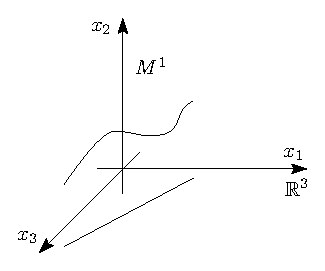
\includegraphics[width=0.35\textwidth]{19_6.eps}
	\caption{Гладкая $1$-мерная поверхность в пространстве.}
	\label{19_6}
\end{figure}

\begin{proof}\hfill\\
	$(\Rightarrow)$  Верно по теореме о неявной функции.
	
	$(\Leftarrow)$ Равенства вида $x = f(y)$ (график функции) можно переписать так: $x -f(y) = 0$ (множество уровня отображения), то есть локально поверхность задается $(n-k)$ уравнениями. Применяем предыдущее утверждение и получаем требуемое.
\end{proof}
\begin{rem}
	Рассмотрим снова определение гладкой $k$-мерной поверхности. Обозначим в нем:
	$$
		V(0) \cap \{u_{k+1} = \dotsc = u_n = 0\} = W \subset \MR^k
	$$
	$W$ это открытое множество в $\MR^k$ (открытая окрестность нуля в пространстве $\MR^k$) в котором находятся координаты $u_1, \dotsc, u_k$. Рассмотрим обратное отображение $f^{-1}$, оно задается как 
	$$
		f^{-1}(u_1,\dotsc,u_k, u_{k+1}, \dotsc, u_n) \colon V \to Q
	$$ 
	Занулим последние $(n-k)$ координат и введем функцию $g$:
	$$
		g = f^{-1}(u_1,\dotsc,u_k, 0, \dotsc, 0) \Rightarrow g\colon W \to \MR^n, \, g(W) = Q \cap M^k
	$$
	Следовательно, кусок поверхности $M^k \cap Q$ можно воспринимать так: есть $k$ параметров: $u_1,\dotsc, u_k$, которые бегают в пространстве $\MR^k$ по некоторому открытому множеству и есть зависимость:
	$$
		g\colon \left\{
		\begin{array}{ccc}
			x_1& = &x_1(u_1,\dotsc, u_k) \\
			\vdots & \vdots & \vdots \\
			x_n& = &x_n(u_1,\dotsc, u_k)
		\end{array}\right.
	$$
	и когда эти $k$ параметров меняются, то рисуется множество в $\MR^n$. Получается параметрически заданная часть поверхности. Более того, $g$ является непрерывно дифференцируемой функцией (как обратное к диффеоморфизму).
	\begin{figure}[H]
		\centering
		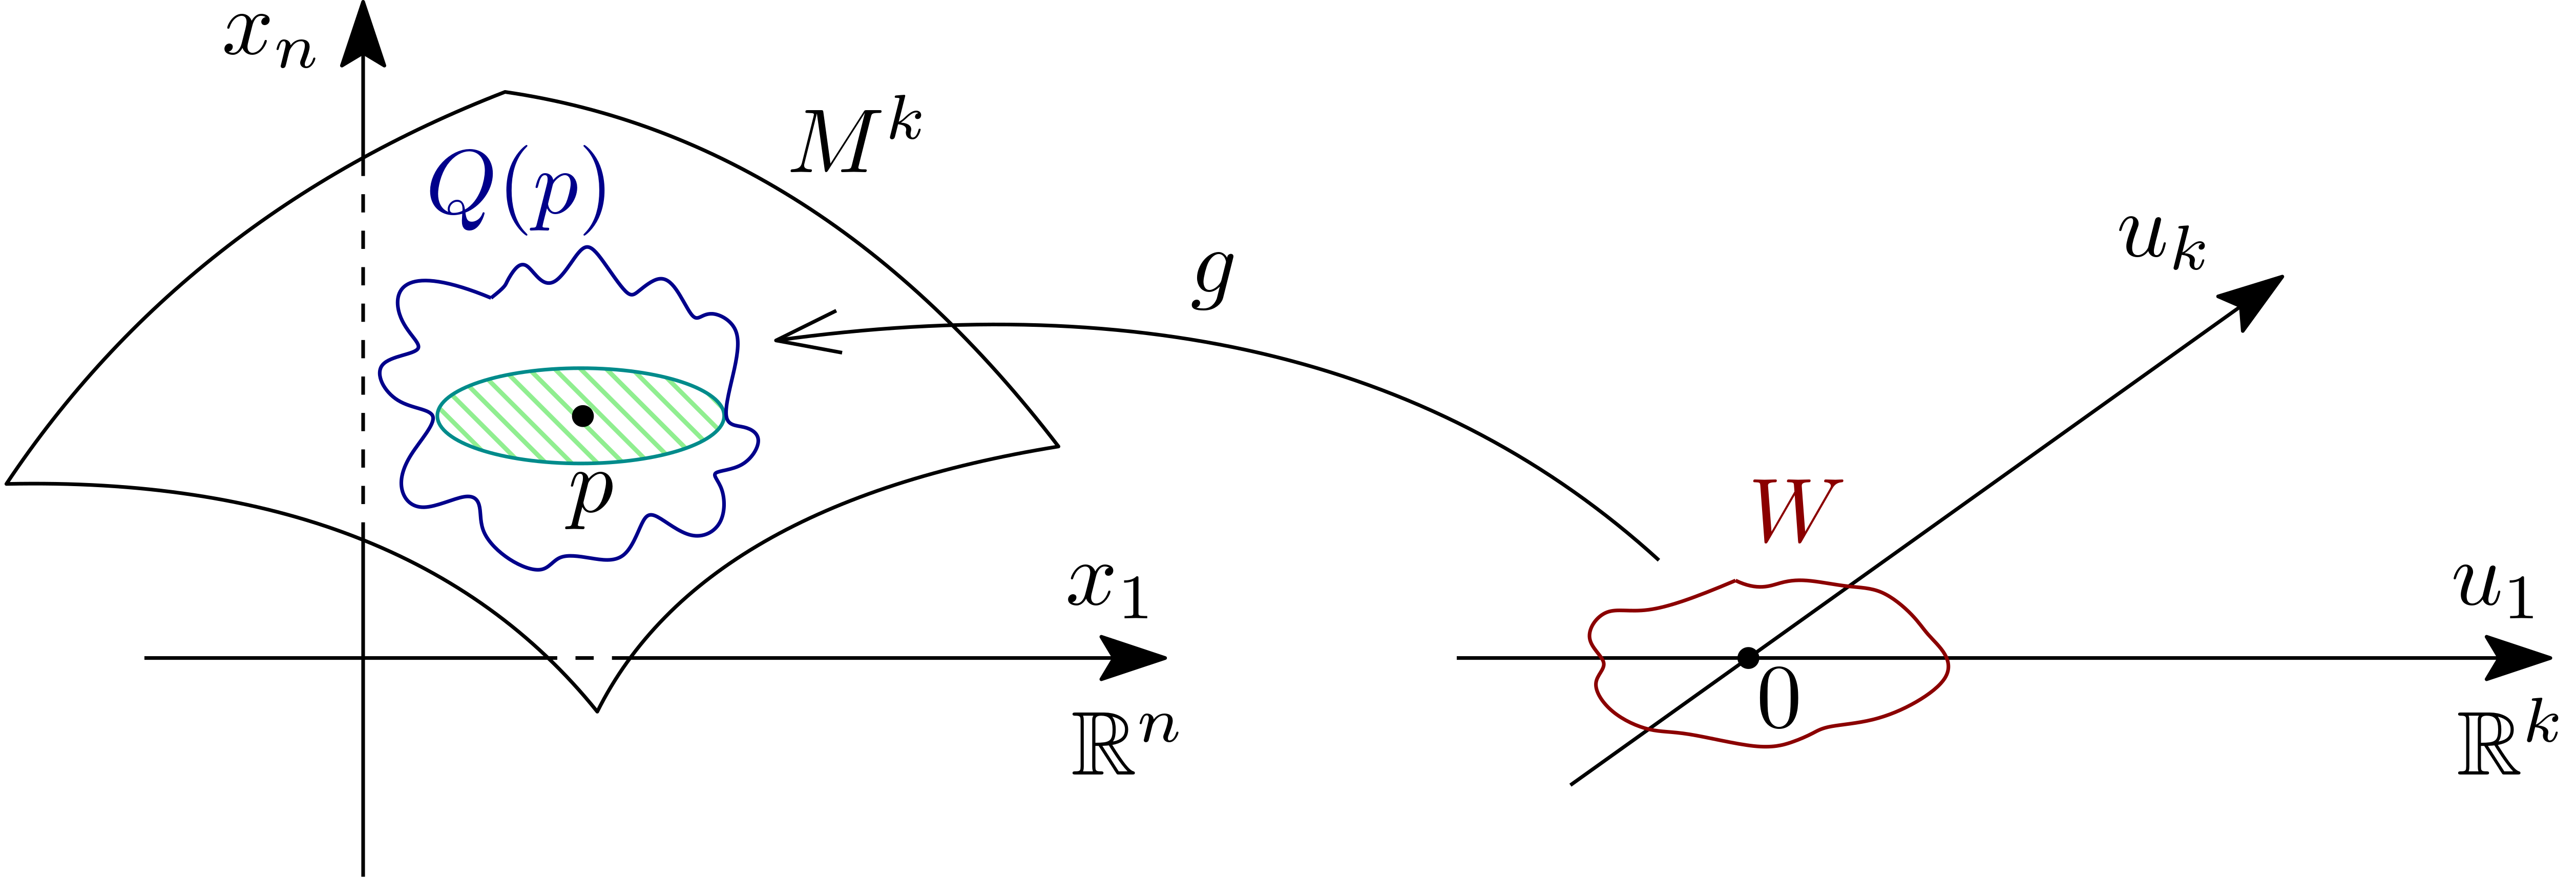
\includegraphics[width=0.75\textwidth]{19_7.png}
		\caption{Отображение $g$ параметризует кусок окрестности, который лежит в $Q$.}
		\label{19_7}
	\end{figure}
	Также отметим, что ранг матрицы Якоби этого отображения равен $k$: 
	$$
		\rk J_g = \rk \begin{pmatrix}
			\tfrac{\partial x_1}{\partial u_1} & \dotsc & \tfrac{\partial x_1}{\partial u_k}\\
			\vdots & \ddots & \vdots \\
			\tfrac{\partial x_n}{\partial u_1} & \dotsc & \tfrac{\partial x_n}{\partial u_k}
		\end{pmatrix}  = k
	$$
	в силу того, что мы взяли обратное отображение к диффеоморфизму (оно невырожденное). В противном случае, если бы среди этих $k$ столбцов оказались линейно зависимые, то ранг матрицы Якобои отображения $f^{-1} \colon  x = x(u)$ был бы меньше $n$:
	$$
		\rk J_{f^{-1}} = \rk \begin{pmatrix}
			\tfrac{\partial x_1}{\partial u_1} & \dotsc & \tfrac{\partial x_1}{\partial u_k} & \tfrac{\partial x_1}{\partial u_{k+1}} & \dotsc & \tfrac{\partial x_1}{\partial u_n}\\
			\vdots & \ddots & \vdots & \vdots & \ddots & \vdots \\
			\tfrac{\partial x_n}{\partial u_1} & \dotsc & \tfrac{\partial x_n}{\partial u_k}  & \tfrac{\partial x_n}{\partial u_{k+1}} & \dotsc & \tfrac{\partial x_n}{\partial u_n}
		\end{pmatrix}  < n
	$$
	А это противоречило бы определению диффеоморфизма (матрица была бы вырожденная). В результате, поверхность задается параметрически $k$ параметрами, но они должны быть независимы друг от друга.
\end{rem}
Теперь в задаче об условном экстремуме мы можем спокойно сказать, где же мы исследуем функцию на условный экстремум - мы будем исследовать её на гладкой $k$-мерной поверхности. Но нам понадобится ещё один объект, связанный с поверхностями - касательное пространство.

\newpage
\section*{Касательное пространство}
Пусть есть поверхность $M^k$. Как нам сказать, что в точке $p$ её что-то касается? Начнем с более простой задачи. Пусть у нас есть кривая $\gamma(t) \colon (-1,1) \to \MR^n$ (одномерная поверхность). Что естественно считать касанием этой кривой в какой-то точке? Вектор скорости. Естественно думать что этот вектор задает натянутую на него прямую, которая как раз и касается кривой $\gamma(t)$  в точке.
\begin{figure}[H]
	\centering
	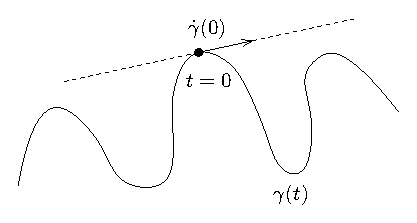
\includegraphics[width=0.35\textwidth]{19_8.eps}
	\caption{Вектор скорости в точке $t = 0$ кривой $\gamma(t)$.}
	\label{19_8}
\end{figure}
Будем считать что интуитивно понятно: если нарисовали кривую, то вектор скорости $\dot{\gamma}(t_0)$ объявляется касательным к этой кривой. Из этого легко объяснить что является касательной плоскостью.

Касательное пространство это линейное пространство. Что объявить векторами, которые касаются в точке $p$ поверхности $M^k$? Проведем через эту точку кривую $\gamma$ так, чтобы в точке $p$ это было $\gamma(0)$ и просто будем вычислять вектор скорости $\dot{\gamma}$ и именно его объявим касательным вектором. Все вместе эти вектора должны образовать касательное пространство.
\begin{figure}[H]
	\centering
	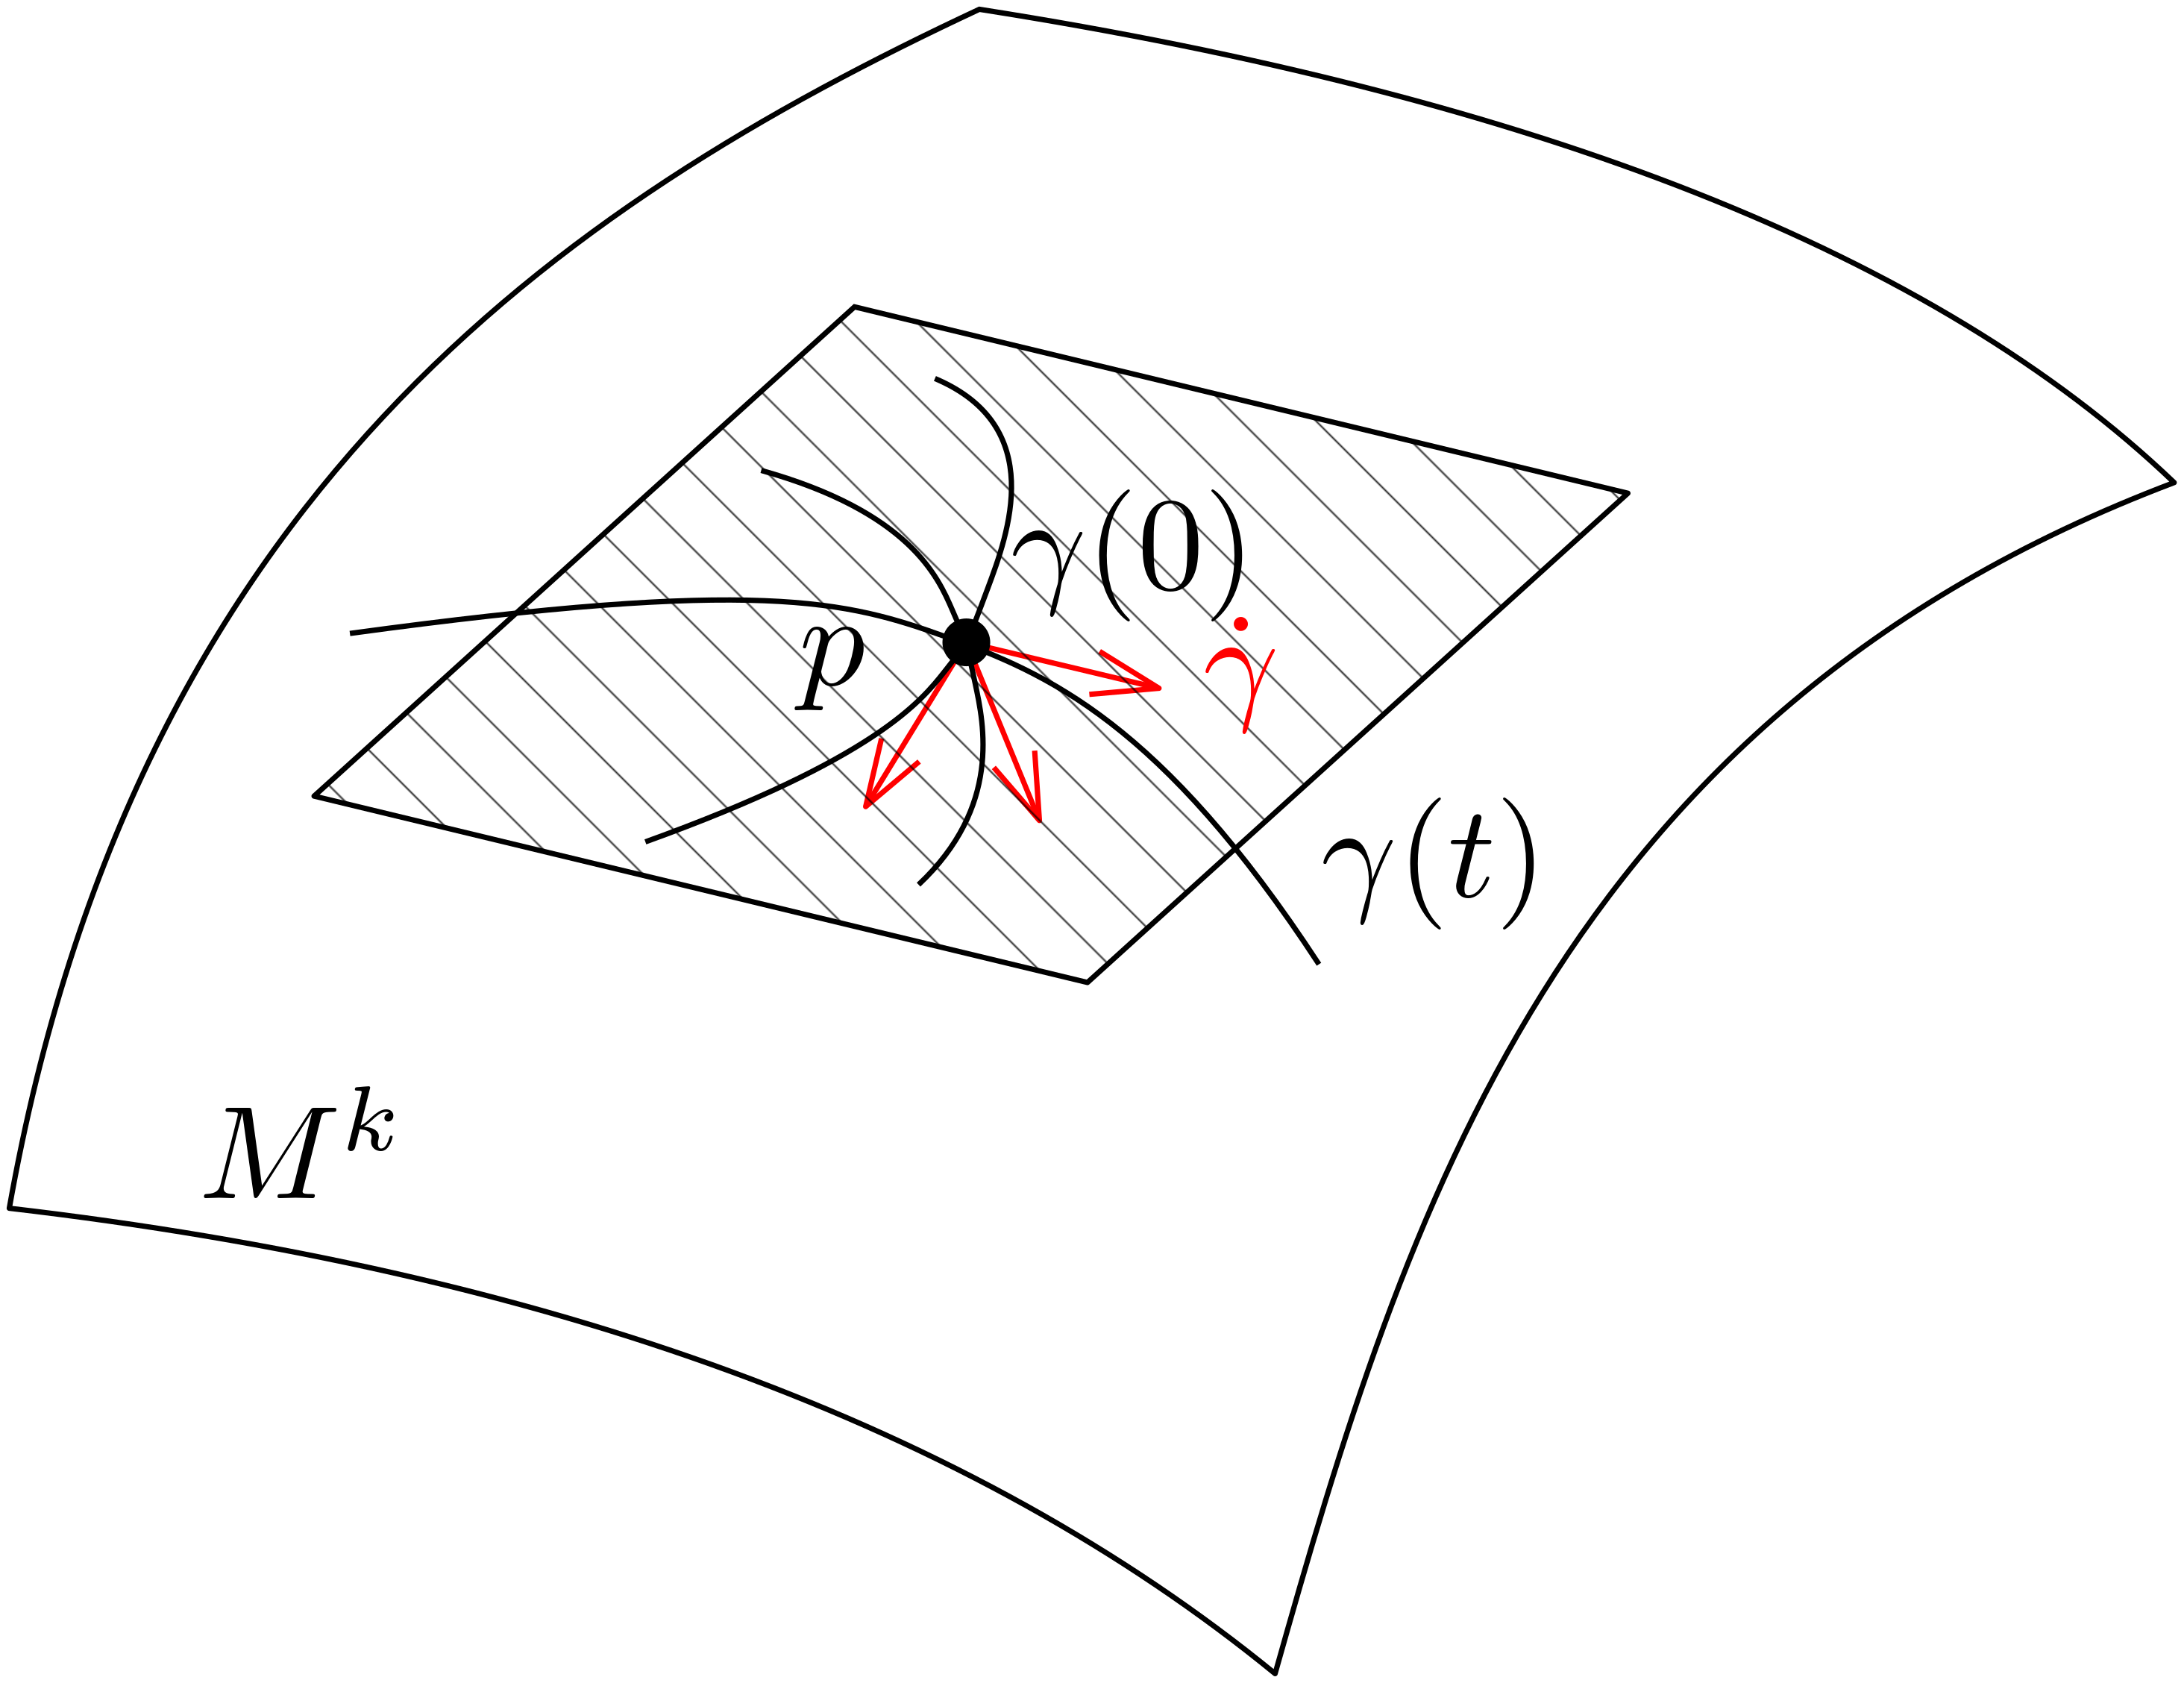
\includegraphics[width=0.35\textwidth]{19_9.png}
	\caption{Касательное пространство.}
	\label{19_9}
\end{figure}
\begin{defn}
	Пусть $M^k$ - гладкая $k$-мерная поверхность в $\MR^n$, $p \in M^k$. \uwave{Касательным пространством} $T_pM^k$ \uwave{в точке} $p$ будем называть множество:
	$$
		T_pM^k = \{v \in \MR^n \mid \exists \, \gamma \colon (-1,1) \to \MR^n, \gamma(t) \in C(-1,1), \,  \gamma(t) \in M^k, \, \gamma(0) = p, \, \dot{\gamma}(0) = v\}
	$$
	где $\gamma(t) \in C(-1,1)$ означает что $\gamma(t)$ - гладкая кривая, то есть непрерывно дифференцируема на $(-1,1)$.
\end{defn}
\begin{prop}
	$T_p M^k$ это $k$-мерное линейное пространство.
\end{prop}
\begin{proof}
	Пусть есть поверхность $M^k$, точка $p \in M^k$ и мы провели кривую $\gamma(t)$ через эту точку. Возьмем диффеоморфизм $f$, определяющий в окрестности точки $p$ (в окрестности $Q$, где есть отображение) поверхность $M^k$. Тогда в координатах плоскости $u_1,\dotsc, u_k$ мы получим проходящую через ноль гладкую кривую $u(t) = f\big(\gamma(t)\big)$ (поскольку $f$ - диффеоморфизм). И наоборот, взяв кривую $u(t)$ и вернувшись в $M^k$ отображением $g$ (тем самым, которое задает параметризацию) получим $\gamma(t) = g\big(u(t)\big)$.
	\begin{figure}[H]
		\centering
		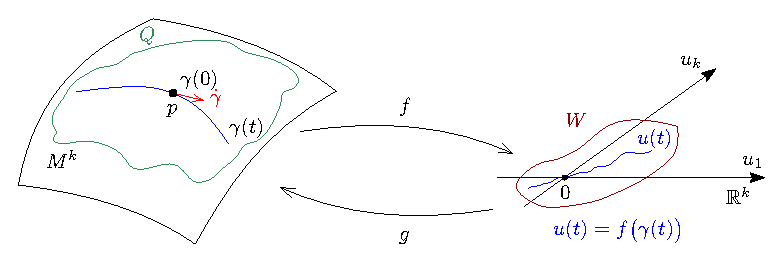
\includegraphics[width=0.65\textwidth]{19_10.eps}
		\caption{Эквивалентность гладких кривых в $W$ и $Q$.}
		\label{19_10}
	\end{figure}
	 Таким образом, рисовать гладкие кривые, проходящие через точку $p$ на поверхности это то же самое, что брать гладкую кривую $u(t)$, проходящую через точку $0$ в открытом множестве $W$ и затем применять отображение $g$, которое параметризуют соответствующий кусок поверхности. Таким образом получили отображение $\gamma(t)$:
	 $$
	 	\gamma(t)\colon \left\{
	 	\begin{array}{ccc}
	 		x_1& = &x_1\big(u_1(t),\dotsc, u_k(t)\big) \\
	 		\vdots & \vdots & \vdots \\
	 		x_n& = &x_n\big(u_1(t),\dotsc, u_k(t)\big)
	 	\end{array}\right.
	 $$
	 
	 Посчитаем вектор скорости в точке $0$:
	 $$
	 	\dot{\gamma}(0)\colon \left\{
	 	\begin{array}{c}
	 		\dfrac{\partial x_1}{\partial u_1}\dot{u}_1(0) + \dotsc +  \dfrac{\partial x_1}{\partial u_k}\dot{u}_k(0)\\
		 	\vdots \\
	 		\dfrac{\partial x_n}{\partial u_1}\dot{u}_1(0) + \dotsc +  \dfrac{\partial x_n}{\partial u_k}\dot{u}_k(0)
	 	\end{array}\right. \Rightarrow
	 	\dot{\gamma}(0) = \dot{u}_1(0){\cdot}\!\!
	 	\begin{pmatrix}
			\dfrac{\partial x_1}{\partial u_1}\\
			\vdots\\
			\dfrac{\partial x_n}{\partial u_1}
	 	\end{pmatrix} 
	 	+ \dotsc + \dot{u}_k(0){\cdot}\!\!
		 \begin{pmatrix}
	 		\dfrac{\partial x_1}{\partial u_k}\\
	 		\vdots\\
	 		\dfrac{\partial x_n}{\partial u_k}
	 	\end{pmatrix}
	 $$
	 Если мы возьмем в качестве $u(t)$ функцию следующего вида:
	 $$
	 	u(t) = \begin{pmatrix}
	 		\underset{1}{0} & \dotsc & \underset{m-1}{0} & \underset{m}{t} & \underset{m+1}{0} & \dotsc & \underset{k}{0}
	 	\end{pmatrix}
	 $$
	 то есть двигаемся вдоль координатной оси $u_m \Rightarrow$ вектор $\dot{\gamma}(0)$ это просто столбец:
	 $$
	 	\dot{\gamma}(0) = \dot{u}_1(0){\cdot}\!\!
	 	\begin{pmatrix}
	 		\dfrac{\partial x_1}{\partial u_1}\\
	 		\vdots\\
	 		\dfrac{\partial x_n}{\partial u_1}
	 	\end{pmatrix} + \dotsc + 
	 	\dot{u}_m(0){\cdot}\!\!	\begin{pmatrix}
	 		\dfrac{\partial x_1}{\partial u_m}\\
	 		\vdots\\
	 		\dfrac{\partial x_n}{\partial u_m}
	 	\end{pmatrix} 
 		+ \dotsc + \dot{u}_k(0){\cdot}\!\!
 		\begin{pmatrix}
 			\dfrac{\partial x_1}{\partial u_k}\\
 			\vdots\\
 			\dfrac{\partial x_n}{\partial u_k}
 		\end{pmatrix} 
 		= 0 + \dotsc +  1{\cdot} \!\! 
		\begin{pmatrix}
			\dfrac{\partial x_1}{\partial u_m}\\
			\vdots\\
			\dfrac{\partial x_n}{\partial u_m} 
		\end{pmatrix} + \dotsc + 0 = 
		\begin{pmatrix}
			\dfrac{\partial x_1}{\partial u_m}\\
			\vdots\\
			\dfrac{\partial x_n}{\partial u_m} 
		\end{pmatrix}
 	= v_m
	 $$
	 Следовательно, это касательный вектор, который получен так: в качестве $\gamma(t)$ взяли образ кривой, которая совпадает с осью координат в координатах $u_1,\dotsc, u_k$. Тогда любой другой касательный вектор есть линейная комбинация этих векторов $v_1, \dotsc, v_k$ или $\dot{\gamma}(0) \in \langle v_1,\dotsc,v_k \rangle$:
	 $$
	 	\dot{\gamma}(0) = c_1v_1 + \dotsc + c_kv_k
	 $$
	 И наоборот, если зададим константы $c_1,\dotsc, c_k$, то предъявим кривую $\gamma$ у которой такой вектор скорости. Если задали набор $(c_1, \dotsc, c_k)$, то в качестве $\gamma(t)$ возьмем то, что получается из кривой $u(t)$ вида:
	 $$
	 	 u(t) = \begin{pmatrix}
	 	 	c_1 t & c_2 t& \dotsc & c_k t
	 	 \end{pmatrix}
	 $$
	 Такой кривой мы опишем движение вдоль вектора $\begin{pmatrix}
	 	c_1 & c_2 & \dotsc & c_k
	 \end{pmatrix}$ на плоскости координат $u_1, \dotsc, u_k$.
	 Получается, что $T_p M^k$ это в точности линейная оболочка векторов $v_1 ,\dotsc, v_k$:
	 $$
	 	T_p M^k = \langle v_1, \dotsc , v_k \rangle
	 $$
	 Это ровно те вектора из которых состояла матрица отображения параметризующего кусок поверхности. Мы говорили, что ранг этой матрицы равен $k \Rightarrow$ линейная оболочка состоит из $k$ линейно независимых векторов. Следовательно, $T_p M^k$ это линейное $k$-мерное пространство.
\end{proof}
\subsection*{Пример в $\MR^3$}
Рассмотрим поверхность $M^2 \subset \MR^3$ и координаты $u_1, u_2$. Отображение $g \colon W \to Q\subset M^2$ параметризует кусок поверхности $M^2$. Возьмем движение вдоль оси $u_1 \Rightarrow$ под действием $g$ через точку $p$ пройдет кривая. Возьмем движение вдоль оси $u_2 \Rightarrow$ под действием $g$ через точку $p$ пройдет еще одна кривая. 

Таким образом, рисуя сетку координат в $W$, мы одновременно рисуем сетку координат (но уже кривую) на поверхности $M^2$. И каждая точка
поверхности однозначно определяется значениями $u_1, u_2$ в системе координат $Ou_1u_2$. Поэтому очень часто $(u_1,u_2)$ называют \uline{локальными координатами}.
\begin{figure}[H]
	\centering
	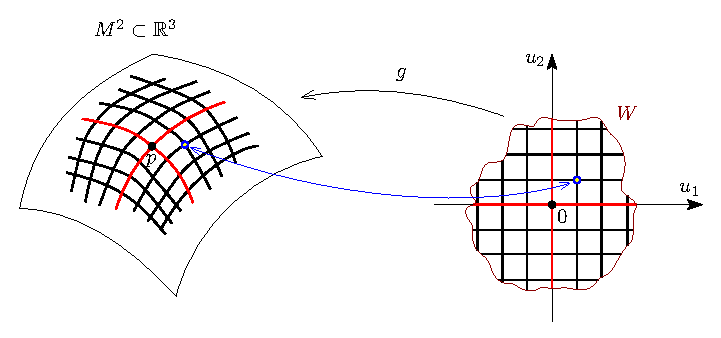
\includegraphics[width=0.65\textwidth]{19_11.eps}
	\caption{Локальные координаты.}
	\label{19_11}
\end{figure}
Уберем сетку и оставим только то, что проходит через точку $p$. Возьмем касательные вектора в этой точке: $\tfrac{\partial x}{\partial u_1}$ и $\tfrac{\partial x}{\partial u_2}$. Любой другой касательный вектор будет выражаться через них. Следовательно, вся касательная плоскость будет натянута на эти два вектора. 

Более того, любой вектор который выразим через $\tfrac{\partial x}{\partial u_1}$ и $\tfrac{\partial x}{\partial u_2}$ можно получить как образ кривой (а на самом деле прямой) линии $\begin{pmatrix}
	c_1 t & c_2 t
\end{pmatrix}$ в $Ou_1u_2$. Тогда $c_1,c_2$ (в силу формулы для вектора скорости) будут коэффициентами перед $\tfrac{\partial x}{\partial u_1}$ и $\tfrac{\partial x}{\partial u_2}$ соответственно. Конкретнее, в доказательстве выше получили:
$$
	\dot{\gamma}(0) = \dot{u}_1(0){\cdot}\!\!
	\begin{pmatrix}
		\dfrac{\partial x_1}{\partial u_1}\\
		\vdots\\
		\dfrac{\partial x_n}{\partial u_1}
	\end{pmatrix} + \dot{u}_2(0){\cdot}\!\!
	\begin{pmatrix}
		\dfrac{\partial x_1}{\partial u_2}\\
		\vdots\\
		\dfrac{\partial x_n}{\partial u_2}
	\end{pmatrix} = \dot{u}_1(0){\cdot}\dfrac{\partial x}{\partial u_1} + \dot{u}_2(0){\cdot}\dfrac{\partial x}{\partial u_2}
$$
Если в качестве $u(t)$ мы возьмем $\begin{pmatrix}t & 0 \end{pmatrix}$, то $\dot{\gamma}(0) = \tfrac{\partial x}{\partial u_1}$, то есть $\tfrac{\partial x}{\partial u_1}$ и $\tfrac{\partial x}{\partial u_2}$ являются касательными векторами, а любой другой касательный вектор является их линейной комбинацией. И наоборот, всякая их линейная комбинация есть касательный вектор \big(должны подобрать $u(t)$ так, чтобы $\dot{u}_1(0) = c_1$ и $\dot{u}_2(0) = c_2$ и, например, подойдет $\begin{pmatrix}c_1 t & c_2 t \end{pmatrix}$\big).

\begin{figure}[H]
	\centering
	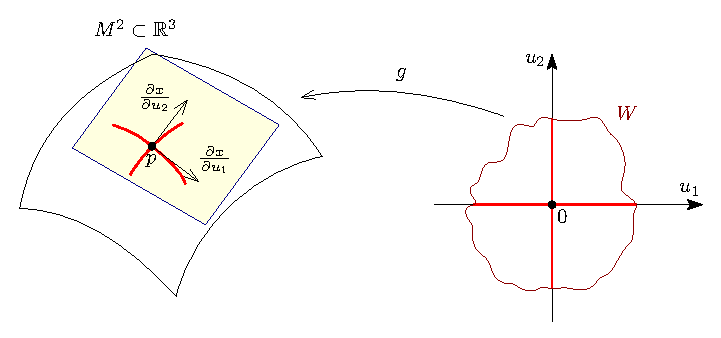
\includegraphics[width=0.65\textwidth]{19_12.eps}
	\caption{Касательная плоскость в точке $p$.}
	\label{19_12}
\end{figure}

\textbf{\uline{Идея}}: Мы взяли вектора, соответствующие движению по осям координат в $Ou_1u_2$ и на них натянули плоскость, которая как раз и будет представлять из себя касательное пространство.

\begin{prop}
	Если $M^k$ в окрестности точки $p$ задается системой уравнений: $F_{k+1}(x) = 0, \dotsc, F_n(x) = 0$, где дифференциалы $dF_{k+1}, \dotsc, dF_n$ - линейно независимы, то касательное пространство есть решение следующей системы уравнений: 
	$$
		v \in T_pM^k \Leftrightarrow 
		\left\{
			\begin{array}{ccc}
				\langle \nabla F_{k+1}(p),v \rangle & =& 0\\
				\vdots & \vdots & \vdots \\
				\langle \nabla F_n(p),v \rangle &=& 0
			\end{array}
		\right.
	$$
\end{prop}
\begin{rem}
	Это уже частично известно нам. Возьмем в $\MR^n$ множество заданное как $F(x) = 0$, то есть множество уровня хорошей функции $F$. Градиент этой функции будет перпендикулярен множеству уровня (соответственно, если двигаемся перпендикулярно градиенту, то значения функции не меняются). 
	
	Теперь это приобретает конкретный смысл: если функция $F$ невырожденная, то $F(x) = 0$ представляет из себя $(n-1)$-мерную поверхность, а вектор градиента становится ортогональным вектором к её касательному пространству. Тогда система уравнений теоремы приобретает вид:
	$$
		T_p M^k = \{v \colon v \perp \nabla F(p)\} = \{v \mid \langle \nabla F(p), v \rangle = 0\}	
	$$
	Касательная плоскость к $F(x) = 0$ в точке $x_0 = p$ это: 
	$$
		\langle x - x_0, \nabla F(x_0) \rangle = 0
	$$ 
	Из аналитической геометрии, чтобы написать к $F(x,y,z) = 0$ касательную плоскость необходимо взять в точке:
	$$
		\dfrac{\partial F}{\partial x}{\cdot}(x - x_0) + \dfrac{\partial F}{\partial y}{\cdot}(y - y_0) + \dfrac{\partial F}{\partial z}{\cdot}(z - z_0) = 0
	$$ 
	и мы получим уравнение касательной плоскости. Это плоскость состоящая из векторов ортогональных градиенту $F$, а значит из векторов принадлежащих касательному пространству (по утверждению выше).
\end{rem}
\begin{proof}
	Пусть $v \in T_p M^k$, мы знаем что $v = \dot{\gamma}(0)$ для гладкой кривой, лежащей в $M^k$. Если кривая $\gamma \in M^k$, то $F_{k+1}\big(\gamma(t)\big) = 0, \dotsc, F_{n}\big(\gamma(t)\big) = 0$. Продифференцируем эту систему в точке $t = 0$:
	$$
		\left\{
			\begin{array}{ccccc}
				\dfrac{d}{dt} F_{k+1}\big(\gamma(t)\big)\bigg|_{t = 0} & =& 0 & = & \langle \nabla F_{k+1}(p),\dot{\gamma}(0) \rangle\\
				\vdots & \vdots & \vdots  & \vdots & \vdots \\
				\dfrac{d}{dt} F_{n}\big(\gamma(t)\big)\bigg|_{t = 0} &=& 0 & = & \langle \nabla F_{n}(p),\dot{\gamma}(0) \rangle
			\end{array}
		\right.
	$$
	где $\gamma(0) = p$. То есть $T_p M^k$ лежит в пространстве решений системы уравнений:
	$$
				\left\{
		\begin{array}{ccc}
			\langle \nabla F_{k+1}(p),v \rangle & =& 0\\
			\vdots & \vdots & \vdots \\
			\langle \nabla F_n(p),v \rangle &=& 0
		\end{array}
		\right.
	$$
	Эта система в свою очередь состоит из $n-k$ невырожденных уравнений. Размерность пространства решений однородной системы из $n-k$ уравнений это $k$. Одно $k$-мерное пространство лежит в другом, но так может быть только если они совпадают.
\end{proof}

\end{document}